\documentclass[11pt,]{article}
\usepackage{lmodern}
\usepackage{amssymb,amsmath}
\usepackage{ifxetex,ifluatex}
\usepackage{fixltx2e} % provides \textsubscript
\ifnum 0\ifxetex 1\fi\ifluatex 1\fi=0 % if pdftex
  \usepackage[T1]{fontenc}
  \usepackage[utf8]{inputenc}
\else % if luatex or xelatex
  \ifxetex
    \usepackage{mathspec}
  \else
    \usepackage{fontspec}
  \fi
  \defaultfontfeatures{Ligatures=TeX,Scale=MatchLowercase}
\fi
% use upquote if available, for straight quotes in verbatim environments
\IfFileExists{upquote.sty}{\usepackage{upquote}}{}
% use microtype if available
\IfFileExists{microtype.sty}{%
\usepackage{microtype}
\UseMicrotypeSet[protrusion]{basicmath} % disable protrusion for tt fonts
}{}
\usepackage[margin=1.0in]{geometry}
\usepackage{hyperref}
\hypersetup{unicode=true,
            pdfborder={0 0 0},
            breaklinks=true}
\urlstyle{same}  % don't use monospace font for urls
\usepackage{graphicx,grffile}
\makeatletter
\def\maxwidth{\ifdim\Gin@nat@width>\linewidth\linewidth\else\Gin@nat@width\fi}
\def\maxheight{\ifdim\Gin@nat@height>\textheight\textheight\else\Gin@nat@height\fi}
\makeatother
% Scale images if necessary, so that they will not overflow the page
% margins by default, and it is still possible to overwrite the defaults
% using explicit options in \includegraphics[width, height, ...]{}
\setkeys{Gin}{width=\maxwidth,height=\maxheight,keepaspectratio}
\IfFileExists{parskip.sty}{%
\usepackage{parskip}
}{% else
\setlength{\parindent}{0pt}
\setlength{\parskip}{6pt plus 2pt minus 1pt}
}
\setlength{\emergencystretch}{3em}  % prevent overfull lines
\providecommand{\tightlist}{%
  \setlength{\itemsep}{0pt}\setlength{\parskip}{0pt}}
\setcounter{secnumdepth}{0}
% Redefines (sub)paragraphs to behave more like sections
\ifx\paragraph\undefined\else
\let\oldparagraph\paragraph
\renewcommand{\paragraph}[1]{\oldparagraph{#1}\mbox{}}
\fi
\ifx\subparagraph\undefined\else
\let\oldsubparagraph\subparagraph
\renewcommand{\subparagraph}[1]{\oldsubparagraph{#1}\mbox{}}
\fi

%%% Use protect on footnotes to avoid problems with footnotes in titles
\let\rmarkdownfootnote\footnote%
\def\footnote{\protect\rmarkdownfootnote}

%%% Change title format to be more compact
\usepackage{titling}

% Create subtitle command for use in maketitle
\newcommand{\subtitle}[1]{
  \posttitle{
    \begin{center}\large#1\end{center}
    }
}

\setlength{\droptitle}{-2em}

  \title{}
    \pretitle{\vspace{\droptitle}}
  \posttitle{}
    \author{}
    \preauthor{}\postauthor{}
    \date{}
    \predate{}\postdate{}
  
\usepackage{helvet} % Helvetica font
\renewcommand*\familydefault{\sfdefault} % Use the sans serif version of the font
\usepackage[T1]{fontenc}

\usepackage[none]{hyphenat}

\usepackage{setspace}
\doublespacing
\setlength{\parskip}{1em}

\usepackage{lineno}

\usepackage{pdfpages}

\usepackage{amsmath}

\usepackage{mathtools}

\begin{document}

\vspace{25mm}
\begin{center}


\textbf{\huge The impact of DNA polymerase and number of rounds of amplification in PCR on 16S rRNA gene sequence data}

\vspace{50mm}



\textbf{Running title:} Quantifying the effects of PCR conditions

\vspace{25mm}

Marc A Sze${^1}$ and Patrick D Schloss${^1}$${^\dagger}$

\vspace{20mm}

$\dagger$ To whom correspondence should be addressed: pschloss@umich.edu

$1$ Department of Microbiology and Immunology, University of Michigan, Ann Arbor, MI

\end{center}

\newpage
\linenumbers

\hypertarget{abstract}{%
\subsection{Abstract}\label{abstract}}

PCR amplification of 16S rRNA genes is a critical, yet under appreciated
step in the generation of sequence data to describe the taxonomic
composition of microbial communities. Numerous factors in the design of
PCR can impact the sequencing error rate, the abundance of chimeric
sequences, and the degree to which the fragments in the product
represent their abundance in the original sample (i.e.~bias). We
compared the performance of high fidelity polymerases and varying number
of rounds of amplification when amplifying a mock community and human
stool samples. Although it was impossible to derive specific
recommendations, we did observe general trends. Namely, using a
polymerase with the highest possible fidelity and minimizing the number
of rounds of PCR reduced the sequencing error rate, fraction of chimeric
sequences, and bias. Evidence of bias at the sequence level was subtle
and could not be ascribed to the fragments' fraction of bases that were
guanines or cytosines. When analyzing mock community data, the amount
that the community deviated from the expected composition increased with
rounds of PCR. This bias was inconsistent for human stool samples.
Overall the results underscore the difficulty of comparing sequence data
that are generated by different PCR protocols. However, the results
indicate that the variation in human stool samples is generally larger
than that introduced by the choice of polymerase or number of rounds of
PCR.

\hypertarget{importance}{%
\subsubsection{Importance}\label{importance}}

A steep decline in sequencing costs drove an explosion in studies
characterizing microbial communities from diverse environments. Although
a significant amount of effort has gone into understanding the error
profiles of DNA sequencers, little has been done to understand the
downstream effects of the PCR amplification protocol. We quantified the
effects of the choice of polymerase and number of PCR cycles on the
quality of downstream data. We found that these choices can have a
profound impact on the way that a microbial community is represented in
the sequence data. The effects are relatively small compared to the
variation in human stool samples, however, care should be taken to use
polymerases with the highest possible fidelity and to minimize the
number of rounds of PCR. These results also underscore that it is not
possible to directly compare sequence data generated under different PCR
conditions.

\newpage

\hypertarget{introduction}{%
\subsection{Introduction}\label{introduction}}

16S rRNA gene sequencing is a powerful and widely used tool for
surveying the structure of microbial communities (1--3). This approach
has exploded in popularity with the advent of high throughput sequencing
where it is possible to characterize numerous samples with thousands of
sequences per sample. Many factors can impact how a natural community is
represented by the sequencing data including the method of acquiring
samples (4--8), storage conditions (4--6, 9--12), extraction methods
(13), amplification conditions (8, 14, 15), sequencing method (15--17),
and analytical pipeline (15, 18--20). The increased sampling depth that
is now available relative to previous Sanger sequencing-based methods is
expected to compound the impacts of an investigator's choices and the
interpretation of their results.

One step in the generation of 16S rRNA gene sequence data that has been
long known to have a significant impact on the description of microbial
communities is the choice of conditions for PCR amplification (8, 14,
15). Factors such as the choice of primers have an obvious impact on
which populations will be amplified (18, 21). However, a variety of PCR
artifacts can also impact the perception of a community including the
formation of chimeras (14, 22--24), misincorporation of nucleotides (23,
25, 26), preferential amplification of some populations over others
leading to bias (24, 27--33), and accumulation of random amplification
events leading to PCR drift (24, 27, 32, 34). Many bioinformatic tools
have been developed to identify chimeras; however, there are significant
sensitivity and specificity tradeoffs (14, 35). Laboratory-based
solutions to minimize chimera formation have also been proposed such as
minimizing the amount of template DNA in the PCR, minimizing the number
of rounds of PCR, minimizing the amount of shearing in the template DNA,
and using DNA polymerases that have a proof-reading ability (14, 23).
Others have attempted to account for PCR bias using modeling approaches
(29, 36). In cases where there has been success it has been with
relatively small communities with consistent composition (29). To
minimize PCR drift, some investigators pool technical replicate PCRs
hoping to average out the drift (34). Other factors that have been shown
to impact the formation of PCR artifacts are outside the control of an
investigator including the fraction of DNA bases that are guanines or
cytosines, the variation in the length of the targeted region across the
community, the sequence of the DNA that flanks the template, and the
genetic diversity of the community (28, 30--33). Early investigations of
the factors that lead to the formation of PCR artifacts focused on
analyzing binary mixtures of genomic DNA and 16S rRNA gene fragments to
explore PCR biases and chimera formation. Although these studies were
instrumental in forcing researchers to be cautious about the
interpretation of their results, we have a poor understanding of how
these factors affect the formation of PCR artifacts in more complex
communities.

The influence that the choice of DNA polymerase has on the formation of
PCR artifacts has not been well studied. There has been recent interest
in how the choice of the hypervariable region and data analysis
pipelines impact the sequencing error rate (15, 18--20); however, these
studies use the same DNA polymerase in the PCR step and implicitly
assume that the rate of nucleotide misincorporation from PCR are
significantly smaller than those from the sequencing phase. There has
been more limited interest in the impact that DNA polymerase choice has
on the formation of chimeras (23, 37). A recent study found differences
in the number of OTUs and chimeras between normal and high fidelity DNA
polymerases (37). The authors of the study reduced the difference
between two polymerases by optimizing the annealing and extension steps
within the PCR protocol (37). Yet this optimization was specific for the
community they were analyzing (i.e.~captive and semi-captive red-shanked
doucs) and assumed that if the two polymerases generate the same
community structure that the community structure was correct. In fact,
the community structure generated by both methods was not free of
artifacts, but likely had the same artifacts. A challenge in these types
of experiments is having \emph{a priori} knowledge of the true community
representation. A mock community with known composition allows
researchers to quantify the sequencing error rate, fraction of chimeras,
and bias (19); however, mock communities have a limited phylogenetic
diversity relative to natural communities. Natural communities, in
contrast, have an unknown community composition making absolute
measurements impossible. They can be used to validate results from mock
communities and to understand the relative impacts of artifacts on the
ability to differentiate biological and methodological sources of
variation. Given the large number of DNA polymerases available to
researchers, it is unlikely that a specific recommendation is possible.
Rather, the development of general best practices and understanding the
impact of PCR artifacts on an analysis are needed.

This study investigated the impact of choice of high fidelity DNA
polymerase and the number of rounds of amplification on the formation of
PCR artifacts using a mock community and human stool samples. It was
hypothesized that additional rounds of PCR would exacerbate the number
of artifacts. These PCR artifacts included (i) the effect of the
polymerase on the error rate of the bases represented in the final
sequences, (ii) the fraction of sequences that appeared to be chimeras
and the ability to detect those chimeras, (iii) the bias of
preferentially amplifying one fragment over another in a mixed pool of
templates, and (iv) inter-sample variation in community structure of
samples amplified with the same polymerase across the amplification
process. To characterize these factors we sequenced a mock community of
8 organisms with known sequences and community structure and human fecal
samples with unknown sequences and community structures. We sequenced
the V4 region of the 16S rRNA genes from a mock community by generating
paired 250 nt reads on the Illumina MiSeq platform. This region and
sequencing approach was used because it has been shown to result in a
relatively low sequencing error rate and is a widely used protocol (18).
To better understand the impact of DNA polymerase choice on PCR
artifacts, we selected five high fidelity DNA polymerases and amplified
the communities using 20, 25, 30, and 35 rounds of amplification.
Collectively, our results suggest that the number of rounds and to a
lesser extent the choice of DNA polymerase used in PCR impact the
sequence data. The effects are consistent and are smaller than the
biological differences between individuals.

\newpage

\hypertarget{results}{%
\subsection{Results}\label{results}}

\textbf{\emph{Sequencing errors vary by the number of cycles and the DNA
polymerase used in PCR.}} The presence of sequence errors can confound
the ability to accurately classify 16S rRNA gene sequences and group
sequences into operational taxonomic units (OTUs). More importantly,
sequencing errors themselves can alter the representation of the
community. Therefore, it is important to minimize the number of
sequencing errors. Using a widely-used approach that generates the
lowest reported error rate, we quantified the error rate by sequencing
the V4 region of the 16S rRNA genes from an 8 member mock community. We
also removed any contigs that were at least three bases more similar to
a chimera of two references than to a single reference sequence (18, 19,
38). Regardless of the polymerase, the error rate increased with the
number of rounds of amplification (Figure 1). Using 30 rounds of PCR is
a common approach across diverse types of samples. Among the data
generated using 30 rounds of PCR the Accuprime polymerase had the
highest error rate (i.e.~0.124\%) followed by the Platinum
(i.e.~0.094\%), Phusion (i.e.~0.064\%), Kappa (i.e.~0.062\%), and Q5
(i.e.~0.060\%) polymerases (Figure 1). When we applied a pre-clustering
denoising step, which merged the counts of reads within 2 nt of a more
abundant sequence (19), the error rates dropped considerably such that
the Platinum polymerase had the highest error rate (i.e.~0.014\%)
followed by the Accuprime (i.e.~0.012\%), Q5 (i.e.~0.0053\%), Phusion
(i.e.~0.0049\%), and Kappa (i.e.~0.0049\%) polymerases (Figure 1).
Although specific recommendations are difficult to make because the
phylogenetic diversity of the initial DNA template is likely to have an
impact on the results, it is clear that using as few PCR cycles as
necessary and a polymerase with the lowest possible error rate is a good
guide to minimizing the impact of polymerase on the error rate.

\textbf{\emph{The fraction of sequences identified as being chimeric
varies by the number of cycles and the DNA polymerase used in PCR.}}
Chimeric PCR products can significantly confound downstream analyses.
Although numerous bioinformatic tools exist to identify and remove
chimeric sequences with high specificity, their sensitivity is
relatively low and can be reduced by the presence of sequencing errors
(14, 35). Because the true sequences of the organisms in the mock
community were known, we generated all possible chimeras between pairs
of V4 16S rRNA gene fragments and used these possible chimeric sequences
to screen the sequences generated under the different PCR conditions for
chimeras. The number of chimeras increased with rounds of amplification
(Figure 2A). Interestingly, the fraction of chimeric sequences from the
mock community varied by the type of polymerase used. After 30 rounds of
PCR, the Platinum polymerase had the highest chimera rate (i.e.~18.2\%)
followed by the Q5 (i.e.~8.1\%), Phusion (i.e.~7.5\%), Kappa
(i.e.~2.3\%), and Accuprime (i.e.~0.9\%) polymerases. Because our
chimera screening procedure can only be applied to mock communities, we
used the UCHIME algorithm to model the chimera screening approach that
is used in most sequence curation pipelines. By comparing the output of
UCHIME to our reference-based approach, we were able to calculate the
UCHIME's sensitivity and specificity (Figure 2A). The specificity for
all polymerases was above 95.7\% and showed a weak association with the
number of cycles used (Figure 2A). There was considerable
inter-polymerase and inter-round of amplification variation in the
sensitivity of UCHIME to detect the chimeras from the mock community.
This suggested that the residual error rate after pre-clustering the
sequence data did not compromise the sensitivity of UCHIME to detect
chimeras. The sensitivity of UCHIME varied between 50 and 87.0\% when at
least 25 cycles were used. The generalizability of these results is
limited because we used a single mock community with limited genetic
diversity. Although we did not know the true chimera rate for our four
human stool samples, we were able to calculate the fraction of sequences
that UCHIME identified as being chimeric (Figure 2B). These results
followed those from the mock communities: additional rounds of
amplification significantly increased the rate of chimeras and there was
variation between the polymerases that we used. Although it was not
possible to identify the features of a polymerase that resulted in
higher rates of chimeras, it is clear that using the smallest number of
PCR cycles possible will minimize the impact of chimeras.

\textbf{\emph{At the sequence level, PCR amplification bias is subtle.}}
Since researchers began using PCR to amplify 16S rRNA gene fragments
there has been concern that amplifying fragments from a mixed template
pool could lead to a biased representation in the pool of products and
would confound downstream analyses (24, 27--33). The mock community was
generated by mixing equal amounts of genomic DNA from 8 bacteria
resulting in uneven representation of the \emph{rrn} operons across the
bacteria as each bacterium had a different genome size and varied in the
number of operons in its genome. The vendor of the mock community
subjects each lot of genomic DNA to shotgun sequencing to more
accurately quantify the actual abundance of each organism in the
community. We compared the expected relative abundance of the 16S rRNA
genes from each bacterium in the mock community to the data we generated
across rounds of amplification and polymerase (Figure 3). Interestingly,
for some bacteria, their representation became less biased with
additional rounds of PCR (e.g.~\emph{L. fermentum}), while others became
more biased (e.g.~\emph{E. faecalis}), and others had little change
(e.g.~\emph{B. subtilis}). Contrary to prior reports (28), the
percentage of bases in the V4 region that were guanines or cytosines was
not predictive of the amount of bias. Across the strains there was no
variation in the length of their V4 regions and they each had the same
sequence in the region that the primers annealed. One of the bacteria
represented in the mock community, \emph{S. enterica}, had 6 identical
copies of the V4 region and 1 copy that differed from those by one
nucleotide. The dominant copy had a thymidine and the rare copy had a
guanine. We used the sequence data to calculate the ratio of the
dominant to rare variants from \emph{S. enterica} expecting a ratio near
6 (Figure S1). The Accuprime, Phusion, Platinum, and Q5 polymerases
converged to a ratio of 5.4; however, the ratio for the Kappa polymerase
varied between 6.1 and 6.8 for 25 to 35 rounds of PCR. Given the subtle
nature of the variation in the relative abundances of each 16S rRNA gene
fragment, it was not possible to create generalizable rules that would
explain the bias.

\textbf{\emph{At the community level, the effects of PCR amplification
bias grow with additional rounds of PCR.}} Because the variation in bias
between polymerases and across rounds of PCR could be artificially
inflated due to sequencing errors and chimeras, we analyzed the alpha
and beta diversity of the mock community data at different phases of the
sequence curation pipeline (Figure 4). First, we removed the chimeras
from the mock community data as described above and mapped the
individual reads to the OTUs that the 16S rRNA gene fragments would
cluster into if there were no sequencing errors. This gave us a
community distribution that reflected the distribution following PCR
without any artifacts. Although the richness did not change, the Shannon
diversity increased with the number of rounds of PCR for all polymerases
except the Kappa polymerase, for which the diversity decreased (Figure
4A). These data suggest that PCR had the effect of making the community
distribution more even than it was originally, except for the data
generated using the Kappa polymerase where the evenness decreased. Next,
we used the observed sequence errors, but removed chimeras using our
reference-based approach, and clustered the reads to OTUs. The richness
and diversity metrics trended higher with higher error rates and number
of rounds of PCR (Figure 4A). Finally, we used the observed sequence
data and the UCHIME algorithm to identify chimeras. Again, the richness
and diversity metrics trended higher with higher error rates and number
of rounds of PCR (Figure 4A). These comparisons demonstrated that
although the bias at the sequence level was subtle, PCR introduces bias
at the community level that is exacerbated by errors and chimeras when
sequences are clustered into OTUs. When we measured the Bray-Curtis
distance between the communities observed after 25 rounds of
amplification and those at 30 and 35, distances between 25 and 35 rounds
were higher than between 25 and 30 rounds for each of the polymerases by
an average of 0.022 units (Figure 4B). The Platinum polymerase varied
the most across rounds of amplification (25 vs 30 rounds: 0.12; 25 vs 35
rounds: 0.15). Although the distances between samples were small, the
ordination of these distances showed a clear change in community
structure with increasing rounds of PCR (Figure 4C). This observation
was supported by our statistical analysis, which revealed that the
effect of the number of rounds of PCR (R\textsuperscript{2}=0.21,
P\textless{}0.001) was comparable to the choice of polymerase
(R\textsuperscript{2}=0.20, P\textless{}0.001). These results
demonstrate that subtle differences in relative abundances can have an
impact on overall community structure. This variation underscores the
importance of only comparing sequence data that have been generated
using the same PCR conditions.

\textbf{\emph{The choice of polymerase or the number of rounds of
amplification have little impact on the relative interpretation of
community-wide metrics of diversity.}} We expected that the biases that
we observed at the population and community levels using mock community
data would be small relative to the expected differences between
biological samples. To study this further, we calculated alpha and
beta-diversity metrics using the human stool samples for each of the
polymerases and rounds of amplification. We calculated the number of
observed OTUs and Shannon diversity for each condition and stool sample
(Figure 5A). Although there were clear differences between PCR
conditions, the relative ordering of the stool samples did not
meaningfully vary across conditions. When we characterized the variation
between rounds of amplification using human stool samples, the distance
between the 25 and 30 rounds and 25 and 35 rounds varied considerably
between samples and polymerases (Figure 5B). In general the inter-round
variation was lowest for the data generated using the Kappa and
Accuprime polymerases. The data generated using the Platinum polymerase
was consistent across rounds, but overall, it was more biased than the
other polymerases. Considering the average distance across the four
samples varied between 0.39 and 0.56, regardless of the polymerases and
number of rounds of amplification, any bias due to amplification is
unlikely to obscure community-wide differences between samples. In
support of this was our principle coordinates analysis of the
Bray-Curtis distances, which revealed distinct clusters by stool sample
(Figure 5C). Within each cluster there were no obvious patterns related
to the polymerase or number of rounds of PCR. However, our statistical
analysis revealed statistically significant differences in the community
structures with the stool sample explaining the most variation
(R\textsuperscript{2}=0.79, P\textless{}0.001), followed by the number
of rounds of PCR (R\textsuperscript{2}=0.044, P\textless{}0.001) and the
choice of polymerase (R\textsuperscript{2}=0.033, P\textless{}0.001).
Together, these results indicate that for a coarse analysis of
communities, the choice of number of rounds of amplification or
polymerase are not important, but that they must be consistent across
samples. It is difficult to develop a specific recommendation based on
the level of bias across rounds of PCR or polymerases; however, the
general suggestion is to use as few rounds of amplification as possible.

\textbf{\emph{There is little evidence of a relationship between
polymerase or number of rounds of amplification on PCR drift.}} There
have been concerns that the same template DNA subjected to the same PCR
conditions could result in different representations of communities
because of random drift over the course of PCR. To test this, we
determined the average Bray-Curtis distance between replicate reactions
using the same polymerase and number of rounds of amplification (Figure
6). Using the mock community data there were no obvious trends. The
average Bray-Curtis distance within a set of conditions varied by 0.063
to 0.11 units. Although we did not generate technical replicates of each
of the stool samples, the inter-sample variation for each set of
conditions was consistent and varied between 0.50 and 0.56 units. These
data suggest that amplicon sequencing is robust to random variation in
amplification and that any differences are likely to be smaller than
what is considered biologically relevant.

\newpage

\hypertarget{discussion}{%
\subsection{Discussion}\label{discussion}}

Our results suggest that the number of rounds of PCR and to a lesser
degree the choice of DNA polymerase impact the analysis of 16S rRNA gene
sequence data from bacterial communities. Although it was not possible
to make direct connections between PCR conditions and specific sources
of bias, we were able to identify general recommendations that reduce
the amount of error, chimera formation, and bias. Researchers should
strive to minimize the number of rounds of PCR and should use a high
fidelity polymerase. Although specific PCR conditions impact the precise
interpretation of the data, the effects were consistent and were smaller
than the biological differences between the samples we tested. Based on
these observations, amplicons must be generated by consistent protocols
to yield meaningful comparisons. When comparing across studies, values
like richness, diversity, and relative abundances must be made in
relative and not absolute terms.

The observed sequencing error rates and alpha diversity metrics followed
the manufacturers' measurements of their polymerases' fidelity (Figure
1). Accuprime and Platinum have fidelity that are approximately 10-times
higher than that of Taq whereas the fidelity of Phusion, Q5, and Kappa
are more than 100 times higher. Among these polymerases, the Kappa
polymerase resulted in the the lowest error rate, lowest chimera rate,
and least bias across rounds of PCR. Considering polymerase development
is an active area of commercial development with potential new
polymerases becoming available, it is important for researchers to
understand how changing the polymerase impacts downstream analyses for
their type of samples.

Over the past 20 years, a large literature has attempted to document
various PCR biases and underscored the fact that data based on
amplification of DNA from a mixed community are not a true
representation of the actual community. In addition to obvious biases
imposed by primer selection, other factors inherent in PCR can influence
the representation of communities. Factors that can lead to preferential
amplification of one fragment over another have included guanine and
cytosine composition, length, flanking DNA composition, amount of DNA
shearing, and number of rounds of PCR (24, 27--33). In addition,
environmental and reagent contaminants can also have a significant
impact on the analysis of low biomass samples (39). Less well understood
is the effect of phylogenetic diversity on bias and chimera formation.
Communities with low phylogenetic diversity may be more prone to chimera
formation since chimeras are more likely to form among closely related
sequences (14, 35). The interaction of these various influences on PCR
artifacts are complex and difficult to tease apart. Minimizing the level
of DNA shearing and using the fewest number of rounds of PCR with a
polymerase that has the highest possible fidelity are strategies that
can be employed to minimize the formation of chimeras. Although care
should always be taken when choosing a polymerase for 16S rRNA gene
sequencing, our observations show that variation among polymerases is
smaller than the actual biological variation in fecal communities
between individuals.

Even with these strategies it is impossible to remove all PCR artifacts.
Beyond the imperfections of the best polymerases, sometimes difficult to
lyse organisms require stringent lysis steps and low biomass samples
require additional rounds of PCR. A host of bioinformatics tools are
available for removing residual sequencing errors (18, 40--42). These
tools struggle to correctly differentiate true biological diversity
(i.e.~Amplicon Sequencing Variants or ASVs) and PCR or sequencing
errors. Although these methods remove residual errors, they also risk
splitting intragenomic variants into separate ASVs or merging 16S rRNA
gene sequences from different taxa into the same ASV. Other tools are
available for removing chimeras (14, 35) where there is a trade off
between the sensitivity of detecting chimeras and the specificity of
correctly calling a sequence a chimera. In recent years, parameters for
these algorithms have been changed to increase their sensitivity with
little evaluation of the effects on the specificity of the algorithms
(40, 42). Others recommend removing any read that has an abundance below
a specified threshold as a tool to remove PCR and sequencing artifacts
(e.g.~removing all sequences that only appear once) (20, 40--42). This
method must be approached with caution as such approaches are likely to
introduce a different bias of the community representation and ignore
the fact that artifacts may be quite abundant. Ultimately, researchers
must test their hypotheses with multiple methods to validate the claims
they reach with any one method (43). All methods have biases and
limitations and we must use complementary methods to obtain robust
results.

\newpage

\hypertarget{materials-methods}{%
\subsection{Materials \& Methods}\label{materials-methods}}

\textbf{\emph{Mock community.}} The ZymoBIOMICS\textsuperscript{TM}
Microbial Community DNA Standard (Zymo, CA, USA) was used for mock
communities and the bacterial component was made up of \emph{Pseudomonas
aeruginosa}, \emph{Escherichia coli}, \emph{Salmonella enterica},
\emph{Lactobacillus fermentum}, \emph{Enterococcus faecalis},
\emph{Staphylococcus aureus}, \emph{Listeria monocytogenes}, and
\emph{Bacillus subtilis} at equal genomic DNA abundance
(\url{https://web.archive.org/web/20171217151108/http://www.zymoresearch.com:80/microbiomics/microbial-standards/zymobiomics-microbial-community-standards}).
The actual relative abundance for each bacterium was obtained from
Zymo's certificate of analysis for the lot (Lot: ZRC187325), which they
determined using shotgun metagenomic sequencing
(\url{https://github.com/SchlossLab/Sze_PCRSeqEffects_mSphere_2019/data/references/ZRC187325.pdf}).

\textbf{\emph{Human samples.}} Fecal samples were obtained from 4
individuals who were part of an earlier study (44). These samples were
collected using a protocol approved by the University of Michigan
Institutional Review Board. For this study, the samples were
de-identified. DNA was extracted from the fecal samples using the
MOBIO\textsuperscript{TM} PowerMag Microbiome RNA/DNA extraction kit
(now Qiagen, MD, USA).

\textbf{\emph{PCR protocol.}} Five high fidelity DNA polymerases were
tested including AccuPrime\textsuperscript{TM} (ThermoFisher, MA, USA),
KAPA HIFI (Roche, IN, USA), Phusion (New England Biolabs, MA, USA),
Platinum (ThermoFisher, MA, USA), and Q5 (New England Biolabs, MA, USA).
Manufacturer recommendations were followed except for the annealing and
extension times, which were selected based on previously published
protocols (18, 37). Primers targeting the V4 region of the 16S rRNA gene
were used with modifications to generate MiSeq amplicon libraries (18)
(\url{https://github.com/SchlossLab/MiSeq_WetLab_SOP/}). The number of
rounds of PCR used for each sample and polymerase started at 15 and
increased by 5 rounds up to 35 cycles. Insufficient PCR product was
generated using 15 rounds and has not been included in our analysis.

\textbf{\emph{Library generation and sequencing.}} Each PCR condition
(i.e.~combination of polymerase and number of rounds of PCR) were
replicated four times for the mock community and one time for each fecal
sample. Libraries were generated as previously described (18)
(\url{https://github.com/SchlossLab/MiSeq_WetLab_SOP/}). The libraries
were sequenced using the Illumina MiSeq sequencing platform to generate
paired 250-nt reads.

\textbf{\emph{Sequence processing.}} The mothur software program (v
1.41) was used for all sequence processing steps (45). The protocol has
been previously published (18)
(\url{https://www.mothur.org/wiki/MiSeq_SOP}). Briefly, paired reads
were assembled using mothur's make.contigs command to correct errors
introduced by sequencing (18). Any assembled contigs that contained an
ambiguous base call, mapped to the incorrect region of the 16S rRNA
gene, or appeared to be a contaminant were removed from subsequent
analyses. Sequences were further denoised using mothur's pre.cluster
command to merge the counts of sequences that were within 2 nt of a more
abundant sequence. The VSEARCH implementation of UCHIME was used to
screen for chimeras (35, 46). At various stages in the sequence
processing pipeline for the mock community data, the mothur seq.error
command was used to quantify the sequencing error rate as well as the
true chimera rate. This command uses the true sequences from the mock
community to generate all possible chimeras and removes any contigs that
were at least three bases more similar to a chimera than to a reference
sequence. The command then counts the number of substitutions,
insertions, and deletions in the contig relative to the reference
sequence and reports the error rate without the inclusion of chimeric
sequences (19). The reference sequences and operon copy number for each
bacterium were obtained from the ZymoBIOMICS\textsuperscript{TM}
Microbial Community DNA Standard protocol
(\url{https://web.archive.org/web/20181221151905/https://www.zymoresearch.com/media/amasty/amfile/attach/_D6305_D6306_ZymoBIOMICS_Microbial_Community_DNA_Standard_v1.1.3.pdf}).
Sequences were assigned to operational taxonomic units (OTUs) at a
threshold of 3\% dissimilarity using the OptiClust algorithm (47). To
adjust for unequal sequencing when measuring alpha and beta diversity,
all samples were rarefied to 1,000 sequences 1,000 times for downstream
analysis. The Good's coverage for the samples at this level of sampling
was routinely greater than 95\%.

\textbf{\emph{Statistical analysis.}} All analysis was done with the R
(v 3.5.1) software package (48). Data transformation and graphing were
completed using the tidyverse package (v 1.2.1). The distance matrix
data was analyzed using the adonis function within the vegan package (v
2.5.4).

\textbf{\emph{Reproducible methods.}} The data analysis code for this
study can be found at
\url{https://github.com/SchlossLab/Sze_PCRSeqEffects_mSphere_2019}. The
raw sequences are available at the SRA (Accession SRP132931).

\hypertarget{acknowledgements}{%
\subsection{Acknowledgements}\label{acknowledgements}}

We appreciate the willingness of the donors to provide stool samples. We
also thank Judy Opp and April Cockburn for their assistance in
sequencing the samples as part of the Microbiome Core Facility at the
University of Michigan. Additional thanks to members of the Schloss lab
and Dr.~Marcy Balunas for reading earlier drafts of the manuscript and
providing helpful critiques. Support for MAS came from the Canadian
Institute of Health Research and NIH grant UL1TR002240 and support for
PDS came from NIH grants P30DK034933, R01CA215574, and U19AI09087.

\newpage

\hypertarget{references}{%
\subsection{References}\label{references}}

\hypertarget{refs}{}
\leavevmode\hypertarget{ref-Gilbert2018}{}%
1. \textbf{Gilbert JA}, \textbf{Jansson JK}, \textbf{Knight R}. 2018.
Earth microbiome project and global systems biology. mSystems
\textbf{3}.
doi:\href{https://doi.org/10.1128/msystems.00217-17}{10.1128/msystems.00217-17}.

\leavevmode\hypertarget{ref-HMP2012}{}%
2. \textbf{Human Microbiome Consortium}. 2012. Structure, function and
diversity of the healthy human microbiome. Nature \textbf{486}:207--214.
doi:\href{https://doi.org/10.1038/nature11234}{10.1038/nature11234}.

\leavevmode\hypertarget{ref-Schloss2016}{}%
3. \textbf{Schloss PD}, \textbf{Girard RA}, \textbf{Martin T},
\textbf{Edwards J}, \textbf{Thrash JC}. 2016. Status of the archaeal and
bacterial census: An update. mBio \textbf{7}.
doi:\href{https://doi.org/10.1128/mbio.00201-16}{10.1128/mbio.00201-16}.

\leavevmode\hypertarget{ref-Luo2016}{}%
4. \textbf{Luo T}, \textbf{Srinivasan U}, \textbf{Ramadugu K},
\textbf{Shedden KA}, \textbf{Neiswanger K}, \textbf{Trumble E},
\textbf{Li JJ}, \textbf{McNeil DW}, \textbf{Crout RJ}, \textbf{Weyant
RJ}, \textbf{Marazita ML}, \textbf{Foxman B}. 2016. Effects of specimen
collection methodologies and storage conditions on the short-term
stability of oral microbiome taxonomy. Applied and Environmental
Microbiology \textbf{82}:5519--5529.
doi:\href{https://doi.org/10.1128/aem.01132-16}{10.1128/aem.01132-16}.

\leavevmode\hypertarget{ref-Bassis2017}{}%
5. \textbf{Bassis CM}, \textbf{Nicholas M. Moore}, \textbf{Lolans K},
\textbf{Seekatz AM}, \textbf{Weinstein RA}, \textbf{Young VB},
\textbf{Hayden MK}. 2017. Comparison of stool versus rectal swab samples
and storage conditions on bacterial community profiles. BMC Microbiology
\textbf{17}.
doi:\href{https://doi.org/10.1186/s12866-017-0983-9}{10.1186/s12866-017-0983-9}.

\leavevmode\hypertarget{ref-Gorzelak2015}{}%
6. \textbf{Gorzelak MA}, \textbf{Gill SK}, \textbf{Tasnim N},
\textbf{Ahmadi-Vand Z}, \textbf{Jay M}, \textbf{Gibson DL}. 2015.
Methods for improving human gut microbiome data by reducing variability
through sample processing and storage of stool. PLOS ONE
\textbf{10}:e0134802.
doi:\href{https://doi.org/10.1371/journal.pone.0134802}{10.1371/journal.pone.0134802}.

\leavevmode\hypertarget{ref-Dominianni2014}{}%
7. \textbf{Dominianni C}, \textbf{Wu J}, \textbf{Hayes RB}, \textbf{Ahn
J}. 2014. Comparison of methods for fecal microbiome biospecimen
collection. BMC Microbiology \textbf{14}:103.
doi:\href{https://doi.org/10.1186/1471-2180-14-103}{10.1186/1471-2180-14-103}.

\leavevmode\hypertarget{ref-BautistadelosSantos2016}{}%
8. \textbf{Santos QMB-d los}, \textbf{Schroeder JL}, \textbf{Blakemore
O}, \textbf{Moses J}, \textbf{Haffey M}, \textbf{Sloan W}, \textbf{Pinto
AJ}. 2016. The impact of sampling, PCR, and sequencing replication on
discerning changes in drinking water bacterial community over diurnal
time-scales. Water Research \textbf{90}:216--224.
doi:\href{https://doi.org/10.1016/j.watres.2015.12.010}{10.1016/j.watres.2015.12.010}.

\leavevmode\hypertarget{ref-Sinha2015}{}%
9. \textbf{Sinha R}, \textbf{Chen J}, \textbf{Amir A}, \textbf{Vogtmann
E}, \textbf{Shi J}, \textbf{Inman KS}, \textbf{Flores R},
\textbf{Sampson J}, \textbf{Knight R}, \textbf{Chia N}. 2015. Collecting
fecal samples for microbiome analyses in epidemiology studies. Cancer
Epidemiology Biomarkers \& Prevention \textbf{25}:407--416.
doi:\href{https://doi.org/10.1158/1055-9965.epi-15-0951}{10.1158/1055-9965.epi-15-0951}.

\leavevmode\hypertarget{ref-Amir2017b}{}%
10. \textbf{Amir A}, \textbf{McDonald D}, \textbf{Navas-Molina JA},
\textbf{Debelius J}, \textbf{Morton JT}, \textbf{Hyde E},
\textbf{Robbins-Pianka A}, \textbf{Knight R}. 2017. Correcting for
microbial blooms in fecal samples during room-temperature shipping.
mSystems \textbf{2}:e00199--16.
doi:\href{https://doi.org/10.1128/msystems.00199-16}{10.1128/msystems.00199-16}.

\leavevmode\hypertarget{ref-Lauber2010}{}%
11. \textbf{Lauber CL}, \textbf{Zhou N}, \textbf{Gordon JI},
\textbf{Knight R}, \textbf{Fierer N}. 2010. Effect of storage conditions
on the assessment of bacterial community structure in soil and
human-associated samples. FEMS Microbiology Letters \textbf{307}:80--86.
doi:\href{https://doi.org/10.1111/j.1574-6968.2010.01965.x}{10.1111/j.1574-6968.2010.01965.x}.

\leavevmode\hypertarget{ref-Song2016}{}%
12. \textbf{Song SJ}, \textbf{Amir A}, \textbf{Metcalf JL},
\textbf{Amato KR}, \textbf{Xu ZZ}, \textbf{Humphrey G}, \textbf{Knight
R}. 2016. Preservation methods differ in fecal microbiome stability,
affecting suitability for field studies. mSystems \textbf{1}:e00021--16.
doi:\href{https://doi.org/10.1128/msystems.00021-16}{10.1128/msystems.00021-16}.

\leavevmode\hypertarget{ref-Costea2017}{}%
13. \textbf{Costea PI}, \textbf{Zeller G}, \textbf{Sunagawa S},
\textbf{Pelletier E}, \textbf{Alberti A}, \textbf{Levenez F},
\textbf{Tramontano M}, \textbf{Driessen M}, \textbf{Hercog R},
\textbf{Jung F-E}, \textbf{Kultima JR}, \textbf{Hayward MR},
\textbf{Coelho LP}, \textbf{Allen-Vercoe E}, \textbf{Bertrand L},
\textbf{Blaut M}, \textbf{Brown JRM}, \textbf{Carton T},
\textbf{Cools-Portier S}, \textbf{Daigneault M}, \textbf{Derrien M},
\textbf{Druesne A}, \textbf{Vos WM de}, \textbf{Finlay BB},
\textbf{Flint HJ}, \textbf{Guarner F}, \textbf{Hattori M},
\textbf{Heilig H}, \textbf{Luna RA}, \textbf{Hylckama Vlieg J van},
\textbf{Junick J}, \textbf{Klymiuk I}, \textbf{Langella P},
\textbf{Chatelier EL}, \textbf{Mai V}, \textbf{Manichanh C},
\textbf{Martin JC}, \textbf{Mery C}, \textbf{Morita H}, \textbf{O'Toole
PW}, \textbf{Orvain C}, \textbf{Patil KR}, \textbf{Penders J},
\textbf{Persson S}, \textbf{Pons N}, \textbf{Popova M}, \textbf{Salonen
A}, \textbf{Saulnier D}, \textbf{Scott KP}, \textbf{Singh B},
\textbf{Slezak K}, \textbf{Veiga P}, \textbf{Versalovic J}, \textbf{Zhao
L}, \textbf{Zoetendal EG}, \textbf{Ehrlich SD}, \textbf{Dore J},
\textbf{Bork P}. 2017. Towards standards for human fecal sample
processing in metagenomic studies. Nature Biotechnology.
doi:\href{https://doi.org/10.1038/nbt.3960}{10.1038/nbt.3960}.

\leavevmode\hypertarget{ref-Haas2011}{}%
14. \textbf{Haas BJ}, \textbf{Gevers D}, \textbf{Earl AM},
\textbf{Feldgarden M}, \textbf{Ward DV}, \textbf{Giannoukos G},
\textbf{Ciulla D}, \textbf{Tabbaa D}, \textbf{Highlander SK},
\textbf{Sodergren E}, \textbf{Methe B}, \textbf{DeSantis TZ},
\textbf{Petrosino JF}, \textbf{Knight R}, \textbf{and BWB}. 2011.
Chimeric 16S rRNA sequence formation and detection in sanger and
454-pyrosequenced PCR amplicons. Genome Research \textbf{21}:494--504.
doi:\href{https://doi.org/10.1101/gr.112730.110}{10.1101/gr.112730.110}.

\leavevmode\hypertarget{ref-Sinha2017}{}%
15. \textbf{Sinha R}, \textbf{Abu-Ali G}, \textbf{Vogtmann E},
\textbf{Fodor AA}, \textbf{Ren B}, \textbf{Amir A}, \textbf{Schwager E},
\textbf{Crabtree J}, \textbf{Ma S}, \textbf{Abnet CC}, \textbf{Knight
R}, \textbf{White O}, \textbf{Huttenhower C}. 2017. Assessment of
variation in microbial community amplicon sequencing by the microbiome
quality control (MBQC) project consortium. Nature Biotechnology.
doi:\href{https://doi.org/10.1038/nbt.3981}{10.1038/nbt.3981}.

\leavevmode\hypertarget{ref-Meisel2016}{}%
16. \textbf{Meisel JS}, \textbf{Hannigan GD}, \textbf{Tyldsley AS},
\textbf{SanMiguel AJ}, \textbf{Hodkinson BP}, \textbf{Zheng Q},
\textbf{Grice EA}. 2016. Skin microbiome surveys are strongly influenced
by experimental design. Journal of Investigative Dermatology
\textbf{136}:947--956.
doi:\href{https://doi.org/10.1016/j.jid.2016.01.016}{10.1016/j.jid.2016.01.016}.

\leavevmode\hypertarget{ref-Caporaso2010}{}%
17. \textbf{Caporaso JG}, \textbf{Lauber CL}, \textbf{Walters WA},
\textbf{Berg-Lyons D}, \textbf{Lozupone CA}, \textbf{Turnbaugh PJ},
\textbf{Fierer N}, \textbf{Knight R}. 2010. Global patterns of 16S rRNA
diversity at a depth of millions of sequences per sample. Proceedings of
the National Academy of Sciences \textbf{108}:4516--4522.
doi:\href{https://doi.org/10.1073/pnas.1000080107}{10.1073/pnas.1000080107}.

\leavevmode\hypertarget{ref-Kozich2013}{}%
18. \textbf{Kozich JJ}, \textbf{Westcott SL}, \textbf{Baxter NT},
\textbf{Highlander SK}, \textbf{Schloss PD}. 2013. Development of a
dual-index sequencing strategy and curation pipeline for analyzing
amplicon sequence data on the MiSeq illumina sequencing platform.
Applied and Environmental Microbiology \textbf{79}:5112--5120.
doi:\href{https://doi.org/10.1128/aem.01043-13}{10.1128/aem.01043-13}.

\leavevmode\hypertarget{ref-Schloss2011}{}%
19. \textbf{Schloss PD}, \textbf{Gevers D}, \textbf{Westcott SL}. 2011.
Reducing the effects of PCR amplification and sequencing artifacts on
16S rRNA-based studies. PLoS ONE \textbf{6}:e27310.
doi:\href{https://doi.org/10.1371/journal.pone.0027310}{10.1371/journal.pone.0027310}.

\leavevmode\hypertarget{ref-Bokulich2012}{}%
20. \textbf{Bokulich NA}, \textbf{Subramanian S}, \textbf{Faith JJ},
\textbf{Gevers D}, \textbf{Gordon JI}, \textbf{Knight R}, \textbf{Mills
DA}, \textbf{Caporaso JG}. 2012. Quality-filtering vastly improves
diversity estimates from illumina amplicon sequencing. Nature Methods
\textbf{10}:57--59.
doi:\href{https://doi.org/10.1038/nmeth.2276}{10.1038/nmeth.2276}.

\leavevmode\hypertarget{ref-Parada2015}{}%
21. \textbf{Parada AE}, \textbf{Needham DM}, \textbf{Fuhrman JA}. 2015.
Every base matters: Assessing small subunit rRNA primers for marine
microbiomes with mock communities, time series and global field samples.
Environmental Microbiology \textbf{18}:1403--1414.
doi:\href{https://doi.org/10.1111/1462-2920.13023}{10.1111/1462-2920.13023}.

\leavevmode\hypertarget{ref-Wang1996}{}%
22. \textbf{Wang GCY}, \textbf{Wang Y}. 1996. The frequency of chimeric
molecules as a consequence of PCR co-amplification of 16S rRNA genes
from different bacterial species. Microbiology \textbf{142}:1107--1114.
doi:\href{https://doi.org/10.1099/13500872-142-5-1107}{10.1099/13500872-142-5-1107}.

\leavevmode\hypertarget{ref-Potapov2017}{}%
23. \textbf{Potapov V}, \textbf{Ong JL}. 2017. Examining sources of
error in PCR by single-molecule sequencing. PLOS ONE
\textbf{12}:e0169774.
doi:\href{https://doi.org/10.1371/journal.pone.0169774}{10.1371/journal.pone.0169774}.

\leavevmode\hypertarget{ref-Kebschull2015}{}%
24. \textbf{Kebschull JM}, \textbf{Zador AM}. 2015. Sources of
PCR-induced distortions in high-throughput sequencing data sets. Nucleic
Acids Research gkv717.
doi:\href{https://doi.org/10.1093/nar/gkv717}{10.1093/nar/gkv717}.

\leavevmode\hypertarget{ref-McInerney2014}{}%
25. \textbf{McInerney P}, \textbf{Adams P}, \textbf{Hadi MZ}. 2014.
Error rate comparison during polymerase chain reaction by DNA
polymerase. Molecular Biology International \textbf{2014}:1--8.
doi:\href{https://doi.org/10.1155/2014/287430}{10.1155/2014/287430}.

\leavevmode\hypertarget{ref-Cline1996}{}%
26. \textbf{Cline J}. 1996. PCR fidelity of pfu DNA polymerase and other
thermostable DNA polymerases. Nucleic Acids Research
\textbf{24}:3546--3551.
doi:\href{https://doi.org/10.1093/nar/24.18.3546}{10.1093/nar/24.18.3546}.

\leavevmode\hypertarget{ref-Acinas2005}{}%
27. \textbf{Acinas SG}, \textbf{Sarma-Rupavtarm R}, \textbf{Klepac-Ceraj
V}, \textbf{Polz MF}. 2005. PCR-induced sequence artifacts and bias:
Insights from comparison of two 16S rRNA clone libraries constructed
from the same sample. Applied and Environmental Microbiology
\textbf{71}:8966--8969.
doi:\href{https://doi.org/10.1128/aem.71.12.8966-8969.2005}{10.1128/aem.71.12.8966-8969.2005}.

\leavevmode\hypertarget{ref-Polz1998}{}%
28. \textbf{Polz MF}, \textbf{Cavanaugh CM}. 1998. Bias in
template-to-product ratios in multitemplate PCR. Applied and
Environmental Microbiology \textbf{64}:3724--3730.

\leavevmode\hypertarget{ref-Brooks2015}{}%
29. \textbf{Brooks JP}, \textbf{David J Edwards}, \textbf{Harwich MD},
\textbf{Rivera MC}, \textbf{Fettweis JM}, \textbf{Serrano MG},
\textbf{Reris RA}, \textbf{Sheth NU}, \textbf{Huang B}, \textbf{Girerd
P}, \textbf{Strauss JF}, \textbf{Jefferson KK}, \textbf{Buck GA}. 2015.
The truth about metagenomics: Quantifying and counteracting bias in 16S
rRNA studies. BMC Microbiology \textbf{15}.
doi:\href{https://doi.org/10.1186/s12866-015-0351-6}{10.1186/s12866-015-0351-6}.

\leavevmode\hypertarget{ref-Suzuki1996}{}%
30. \textbf{Suzuki MT}, \textbf{Giovannoni SJ}. 1996. Bias caused by
template annealing in the amplification of mixtures of 16S rRNA genes by
PCR. Applied and environmental microbiology \textbf{62}:625--630.

\leavevmode\hypertarget{ref-Chandler1997}{}%
31. \textbf{Chandler D}, \textbf{Fredrickson J}, \textbf{Brockman F}.
1997. Effect of pcr template concentration on the composition and
distribution of total community 16S rDNA clone libraries. Molecular
Ecology \textbf{6}:475--482.

\leavevmode\hypertarget{ref-Wagner1994}{}%
32. \textbf{Wagner A}, \textbf{Blackstone N}, \textbf{Cartwright P},
\textbf{Dick M}, \textbf{Misof B}, \textbf{Snow P}, \textbf{Wagner GP},
\textbf{Bartels J}, \textbf{Murtha M}, \textbf{Pendleton J}. 1994.
Surveys of gene families using polymerase chain reaction: PCR selection
and pcr drift. Systematic Biology \textbf{43}:250--261.

\leavevmode\hypertarget{ref-Hansen1998}{}%
33. \textbf{Hansen MC}, \textbf{Tolker-Nielsen T}, \textbf{Givskov M},
\textbf{Molin S}. 1998. Biased 16S rDNA pcr amplification caused by
interference from dna flanking the template region. FEMS Microbiology
Ecology \textbf{26}:141--149.

\leavevmode\hypertarget{ref-Kennedy2014}{}%
34. \textbf{Kennedy K}, \textbf{Hall MW}, \textbf{Lynch MDJ},
\textbf{Moreno-Hagelsieb G}, \textbf{Neufeld JD}. 2014. Evaluating bias
of illumina-based bacterial 16S rRNA gene profiles. Applied and
Environmental Microbiology \textbf{80}:5717--5722.
doi:\href{https://doi.org/10.1128/aem.01451-14}{10.1128/aem.01451-14}.

\leavevmode\hypertarget{ref-Edgar2011}{}%
35. \textbf{Edgar RC}, \textbf{Haas BJ}, \textbf{Clemente JC},
\textbf{Quince C}, \textbf{Knight R}. 2011. UCHIME improves sensitivity
and speed of chimera detection. Bioinformatics \textbf{27}:2194--2200.
doi:\href{https://doi.org/10.1093/bioinformatics/btr381}{10.1093/bioinformatics/btr381}.

\leavevmode\hypertarget{ref-Edgar2017}{}%
36. \textbf{Edgar RC}. 2017. UNBIAS: An attempt to correct abundance
bias in 16S sequencing, with limited success.
doi:\href{https://doi.org/10.1101/124149}{10.1101/124149}.

\leavevmode\hypertarget{ref-Gohl2016}{}%
37. \textbf{Gohl DM}, \textbf{Vangay P}, \textbf{Garbe J},
\textbf{MacLean A}, \textbf{Hauge A}, \textbf{Becker A}, \textbf{Gould
TJ}, \textbf{Clayton JB}, \textbf{Johnson TJ}, \textbf{Hunter R},
\textbf{Knights D}, \textbf{Beckman KB}. 2016. Systematic improvement of
amplicon marker gene methods for increased accuracy in microbiome
studies. Nature Biotechnology \textbf{34}:942--949.
doi:\href{https://doi.org/10.1038/nbt.3601}{10.1038/nbt.3601}.

\leavevmode\hypertarget{ref-Quince2011}{}%
38. \textbf{Quince C}, \textbf{Lanzen A}, \textbf{Davenport RJ},
\textbf{Turnbaugh PJ}. 2011. Removing noise from pyrosequenced
amplicons. BMC Bioinformatics \textbf{12}:38.
doi:\href{https://doi.org/10.1186/1471-2105-12-38}{10.1186/1471-2105-12-38}.

\leavevmode\hypertarget{ref-Salter2014}{}%
39. \textbf{Salter SJ}, \textbf{Cox MJ}, \textbf{Turek EM},
\textbf{Calus ST}, \textbf{Cookson WO}, \textbf{Moffatt MF},
\textbf{Turner P}, \textbf{Parkhill J}, \textbf{Loman NJ},
\textbf{Walker AW}. 2014. Reagent and laboratory contamination can
critically impact sequence-based microbiome analyses. BMC Biology
\textbf{12}.
doi:\href{https://doi.org/10.1186/s12915-014-0087-z}{10.1186/s12915-014-0087-z}.

\leavevmode\hypertarget{ref-Callahan2016}{}%
40. \textbf{Callahan BJ}, \textbf{McMurdie PJ}, \textbf{Rosen MJ},
\textbf{Han AW}, \textbf{Johnson AJA}, \textbf{Holmes SP}. 2016. DADA2:
High-resolution sample inference from illumina amplicon data. Nature
Methods \textbf{13}:581--583.
doi:\href{https://doi.org/10.1038/nmeth.3869}{10.1038/nmeth.3869}.

\leavevmode\hypertarget{ref-Edgar2016}{}%
41. \textbf{Edgar RC}. 2016. UNOISE2: Improved error-correction for
illumina 16S and ITS amplicon sequencing.
doi:\href{https://doi.org/10.1101/081257}{10.1101/081257}.

\leavevmode\hypertarget{ref-Amir2017a}{}%
42. \textbf{Amir A}, \textbf{McDonald D}, \textbf{Navas-Molina JA},
\textbf{Kopylova E}, \textbf{Morton JT}, \textbf{Xu ZZ},
\textbf{Kightley EP}, \textbf{Thompson LR}, \textbf{Hyde ER},
\textbf{Gonzalez A}, \textbf{Knight R}. 2017. Deblur rapidly resolves
single-nucleotide community sequence patterns. mSystems \textbf{2}.
doi:\href{https://doi.org/10.1128/msystems.00191-16}{10.1128/msystems.00191-16}.

\leavevmode\hypertarget{ref-Schloss2018}{}%
43. \textbf{Schloss PD}. 2018. Identifying and overcoming threats to
reproducibility, replicability, robustness, and generalizability in
microbiome research. mBio \textbf{9}.
doi:\href{https://doi.org/10.1128/mbio.00525-18}{10.1128/mbio.00525-18}.

\leavevmode\hypertarget{ref-Seekatz2016}{}%
44. \textbf{Seekatz AM}, \textbf{Rao K}, \textbf{Santhosh K},
\textbf{Young VB}. 2016. Dynamics of the fecal microbiome in patients
with recurrent and nonrecurrent clostridium difficile infection. Genome
Medicine \textbf{8}.
doi:\href{https://doi.org/10.1186/s13073-016-0298-8}{10.1186/s13073-016-0298-8}.

\leavevmode\hypertarget{ref-Schloss2009}{}%
45. \textbf{Schloss PD}, \textbf{Westcott SL}, \textbf{Ryabin T},
\textbf{Hall JR}, \textbf{Hartmann M}, \textbf{Hollister EB},
\textbf{Lesniewski RA}, \textbf{Oakley BB}, \textbf{Parks DH},
\textbf{Robinson CJ}, \textbf{Sahl JW}, \textbf{Stres B},
\textbf{Thallinger GG}, \textbf{Horn DJV}, \textbf{Weber CF}. 2009.
Introducing mothur: Open-source, platform-independent,
community-supported software for describing and comparing microbial
communities. Applied and Environmental Microbiology
\textbf{75}:7537--7541.
doi:\href{https://doi.org/10.1128/aem.01541-09}{10.1128/aem.01541-09}.

\leavevmode\hypertarget{ref-Rognes2016}{}%
46. \textbf{Rognes T}, \textbf{Flouri T}, \textbf{Nichols B},
\textbf{Quince C}, \textbf{Mahé F}. 2016. VSEARCH: A versatile open
source tool for metagenomics. PeerJ \textbf{4}:e2584.
doi:\href{https://doi.org/10.7717/peerj.2584}{10.7717/peerj.2584}.

\leavevmode\hypertarget{ref-Westcott2017}{}%
47. \textbf{Westcott SL}, \textbf{Schloss PD}. 2017. OptiClust, an
improved method for assigning amplicon-based sequence data to
operational taxonomic units. mSphere \textbf{2}:e00073--17.
doi:\href{https://doi.org/10.1128/mspheredirect.00073-17}{10.1128/mspheredirect.00073-17}.

\leavevmode\hypertarget{ref-r_citation_2018}{}%
48. \textbf{R Core Team}. 2018. R: A language and environment for
statistical computing. R Foundation for Statistical Computing, Vienna,
Austria.

\newpage

\textbf{Figure 1. The error rate of assembled sequence reads increases
with the number of rounds of PCR; however, much of this error was
eliminated by denoising and followed the relative error rates provided
by the manufacturers.}

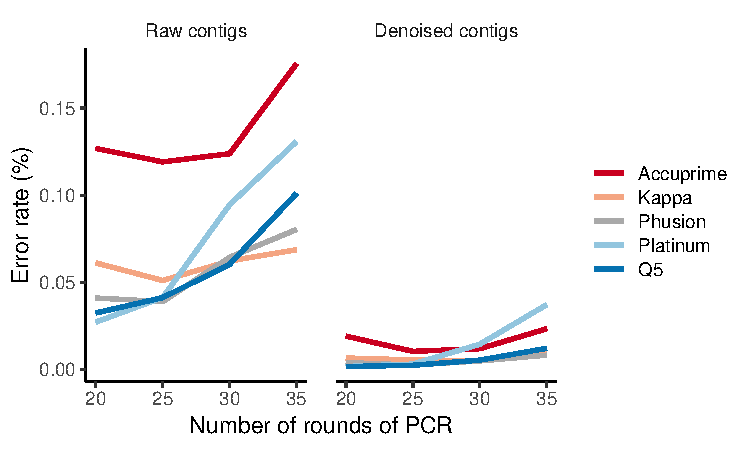
\includegraphics{../results/figures/mock_error.pdf}

\newpage

\textbf{Figure 2. The fraction of all denoised sequences that were
identified as being chimeric increases with the number of rounds of PCR
used and varied between polymerases.} (A) Sequencing of a mock community
allowed us to identify the total fraction of sequences that were
chimeric as well as the sensitivity and specificity of UCHIME to detect
those chimeras. (B) Sequencing of four human stool samples after using
one of five different polymerases again demonstrated increased rate of
chimera formation with increasing number of rounds of PCR and variation
across polymerases.

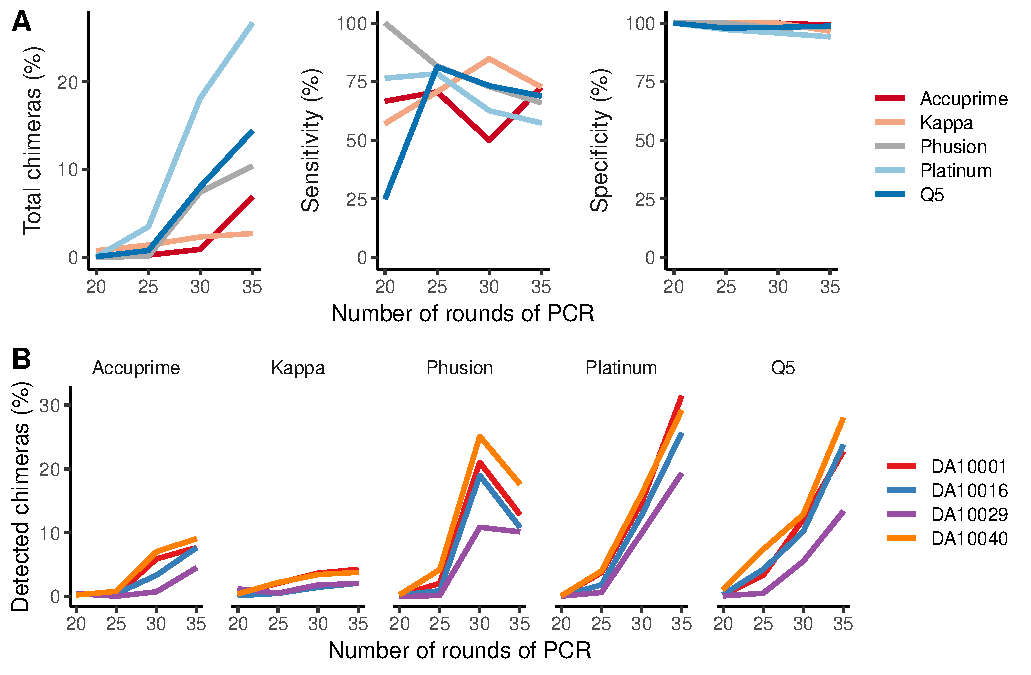
\includegraphics[width=1.0\columnwidth]{../results/figures/chimera_plots.pdf}

\newpage

\textbf{Figure 3. The relative abundances of reads mapped to reference
sequences differed subtly from the expected relative abundances as
determined by shotgun metagenomic sequencing.} Bias did not increase
with number of rounds of PCR or vary by polymerase or the guanine and
cytosine content of the fragment. The expected relative abundance of
each organism is indicated by the horizontal gray line. The percentage
of bases that were guanines or cytosines within the V4 region of the 16S
rRNA genes in each organism is indicated by the number in the lower left
corner of each panel.

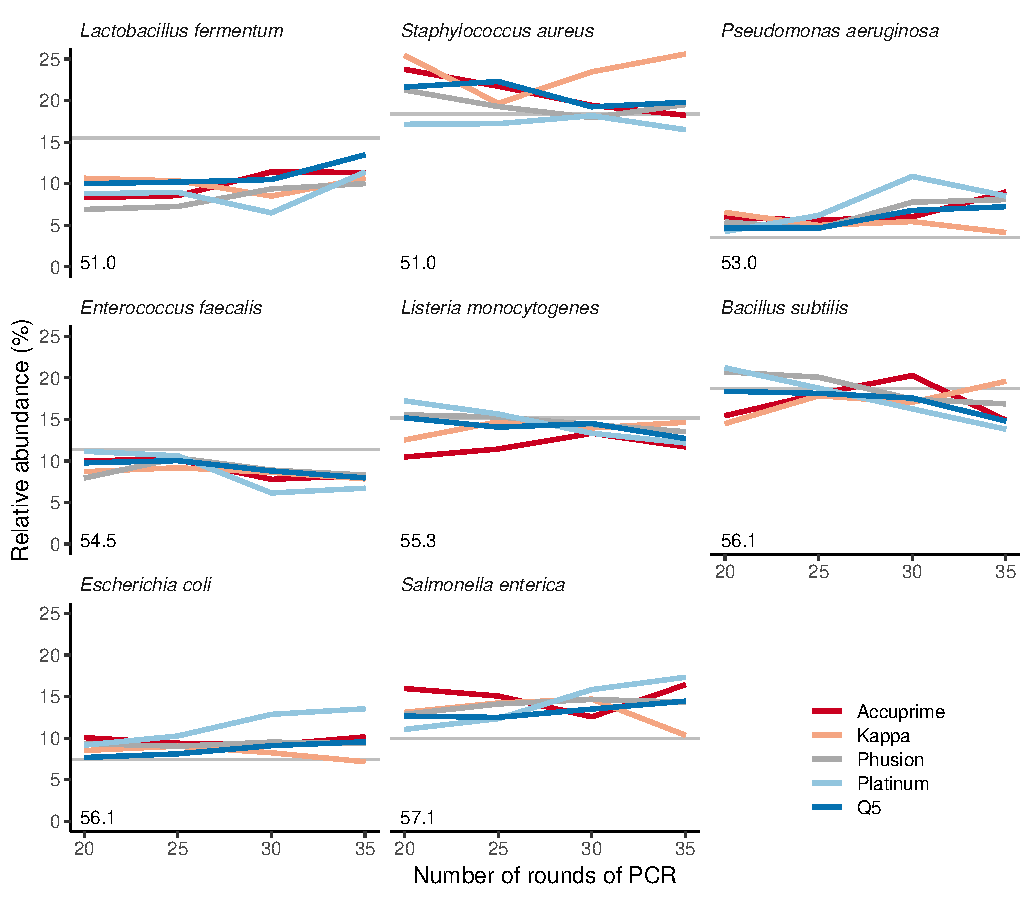
\includegraphics[width=1.0\columnwidth]{../results/figures/species_bias.pdf}

\newpage

\textbf{Figure 4. Despite evidence of subtle PCR bias at the genome
level, there was significant evidence of bias using community-wide
metrics that grew with the number of rounds of PCR when using a mock
community.} (A) With the exception of the Kappa polymerase data, the
richness and Shannon diversity values increased with number of rounds of
PCR and the inclusion of residual sequencing errors and chimeras. The
horizontal black line indicates the expected richness and diversity. (B)
Relative to the mock community sampled after 25 rounds of PCR, the
distance to the communities sampled after 30 and 35 rounds of PCR
increased for all polymerases. (C) The variation between samples
demonstrated a significant change in the community driven by the number
of rounds of PCR and the polymerase used.

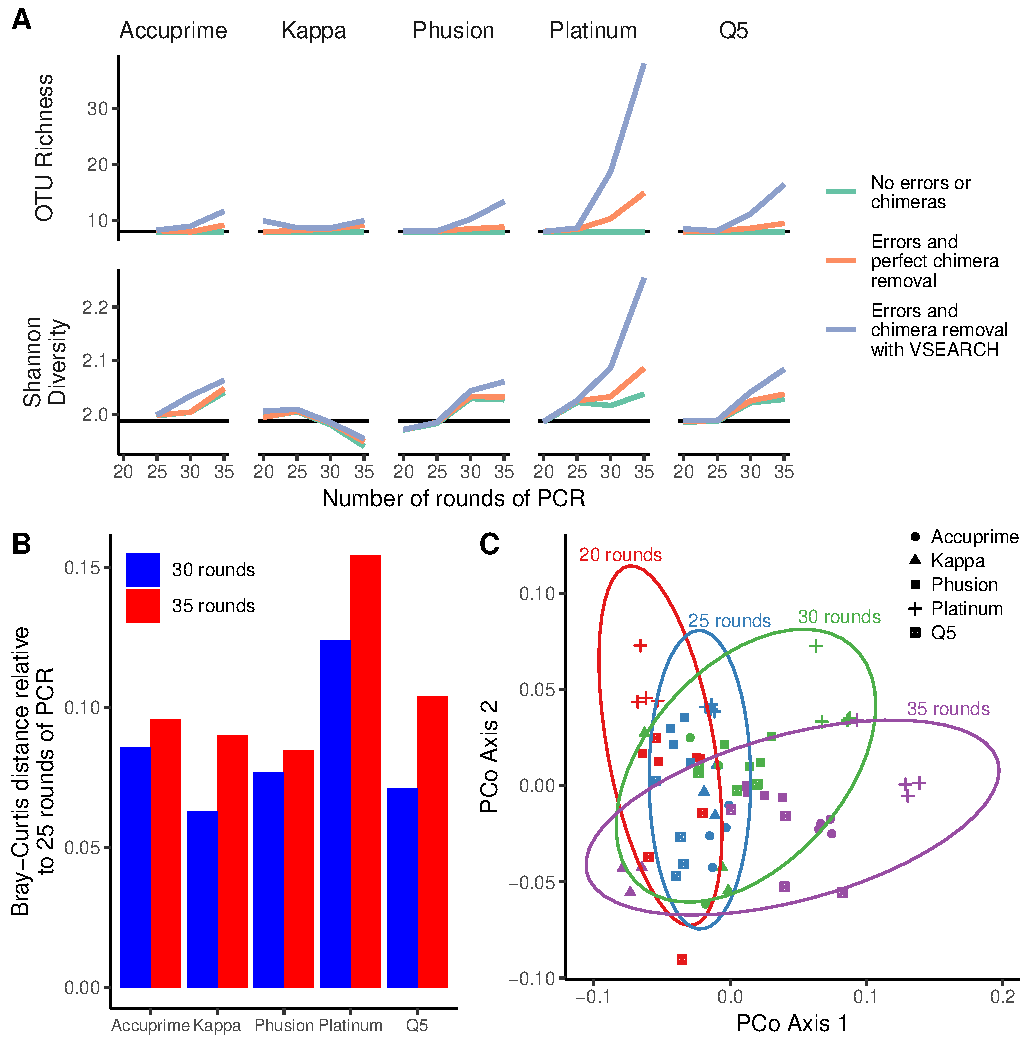
\includegraphics[width=0.9\columnwidth]{../results/figures/mock_community.pdf}

\newpage

\textbf{Figure 5. Sequencing of human stool samples indicated clear
increase in bias with number of rounds of PCR, however, the bias
appeared to be consistent within each sample.} (A) With the exception of
data collected using the Kappa polymerase, the richness and Shannon
diversity values increased with number of rounds of PCR. (B) Relative to
the stool communities sampled after 25 rounds of PCR, the distance to
the stool communities sampled after 30 and 35 rounds of PCR was
inconsistent and there was little difference in variation for data
collected using the Kappa polymerase. (C) The variation between stool
samples was larger than the amount of variation introduced by varying
the number of rounds of PCR or polymerase.

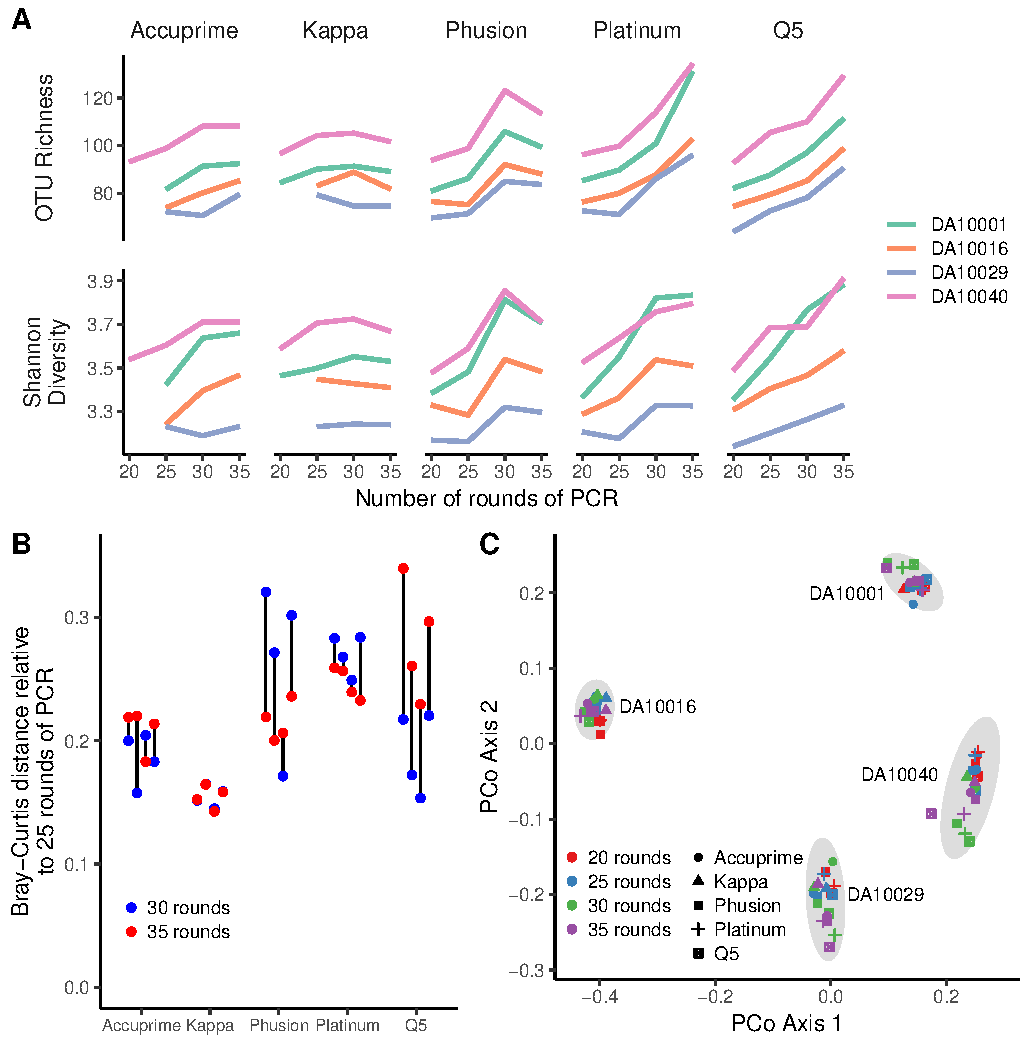
\includegraphics[width=0.9\columnwidth]{../results/figures/stool_community.pdf}

\newpage

\textbf{Figure 6. The average distance between replicates of sequencing
the same mock community or between the the human stool samples
(i.e.~drift) did not vary by number of rounds of PCR or by polymerase.}

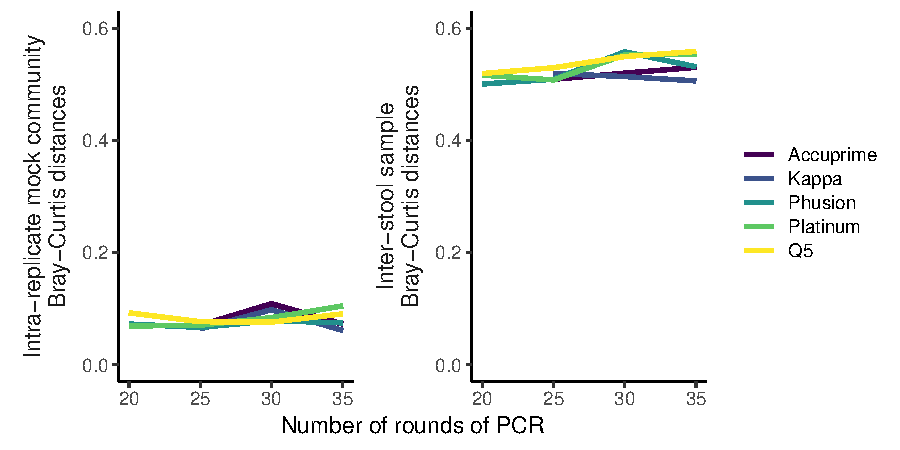
\includegraphics[width=1.0\columnwidth]{../results/figures/drift.pdf}

\newpage

\textbf{Figure S1: With the exception of the sequence data generated
using the Kappa polymerase, the ratio of the two \emph{Salmonella
enterica} V4 sequences was lower than the expected ratio of 6:1.} The
two \emph{S. enterica} V4 sequences differed by a single base.

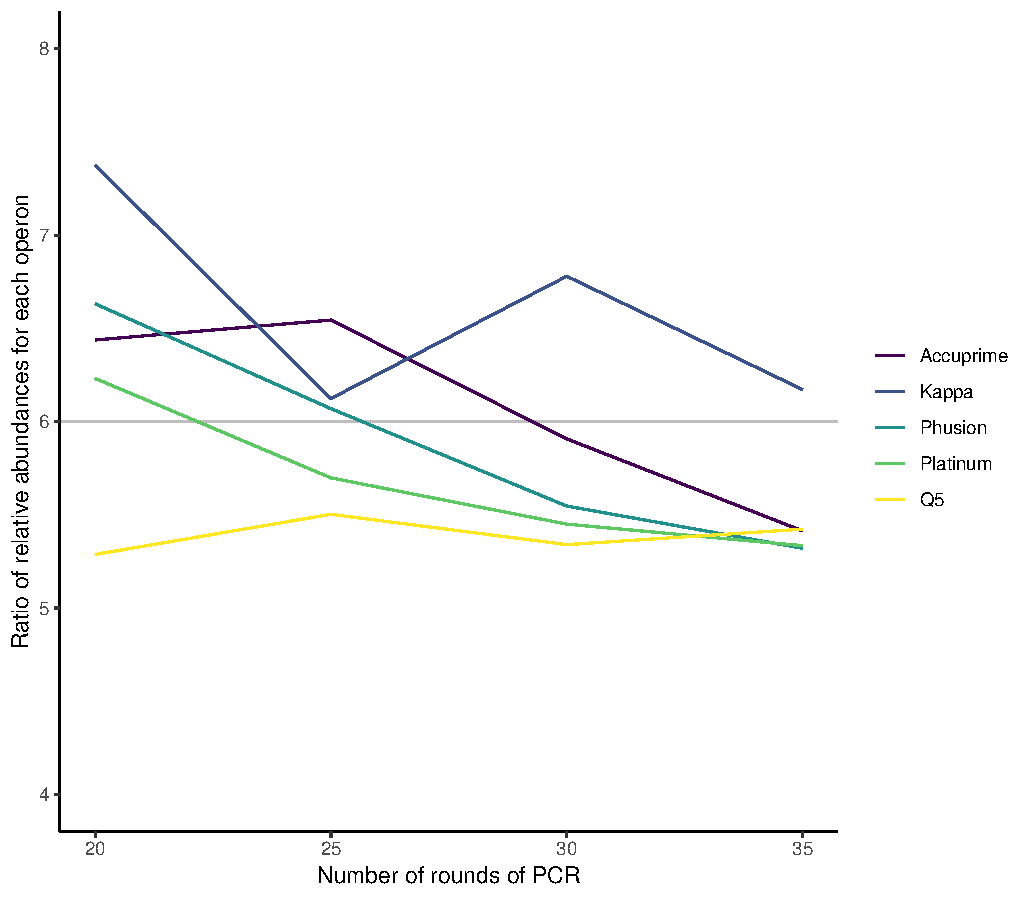
\includegraphics[width=1.0\columnwidth]{../results/figures/salmonella_bias.pdf}


\end{document}
